%
% haar-vater.tex -- Vater-Wavelet für das Haar-Wavelet
%
% (c) 2019 Prof Dr Andreas Müller, Hochschule Rapperswil
%
\documentclass[tikz]{standalone}
\usepackage{amsmath}
\usepackage{times}
\usepackage{txfonts}
\usepackage{pgfplots}
\usepackage{csvsimple}
\usetikzlibrary{arrows,intersections,math}
\begin{document}
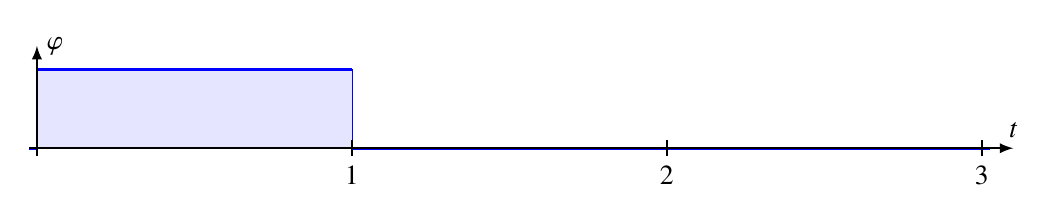
\begin{tikzpicture}[>=latex]

\fill[color=blue!10] (0,0)--(4,0)--(4,1)--(0,1)--cycle;
\draw[line width=1pt,color=blue] (-0.1,0)--(0,0);
\draw[line width=0.1pt,color=blue] (0,0)--(0,1);
\draw[line width=1pt,color=blue] (0,1)--(4,1);
\draw[line width=0.1pt,color=blue] (4,0)--(4,1);
\draw[line width=1pt,color=blue] (4,0)--(12.1,0);

\draw[->,line width=0.7pt] (-0.1,0)--(12.4,0) coordinate[label={$t$}];
\draw[->,line width=0.7pt] (0,-0.1)--(0,1.3) coordinate[label={right:$\varphi$}];

\foreach \x in {1,...,3}{
	\draw[line width=0.7pt] ({4*\x},-0.1)--({4*\x},0.1);
	\node at ({4*\x},-0.1) [below] {$\x$};
}

\end{tikzpicture}
\end{document}

